\subsection{Nested cohorts and target-specific attacks on an NMS-free model}
\label{sec:nested1500}
We recomputed a nested 1,000/1,500-image COCO-val cohort with five starts per image and four attack paths (30,000 image--start attacks). The prefixes are not independent replications. All paths use 100 PGD steps, $\epsilon=16/255$, $\alpha=2/255$, FP32 unfused evaluation, and the final iterate. A zero start and four image-keyed uniform random starts were fixed prospectively. The two target-specific objectives share the same initial perturbation for each image and start.
\begin{table*}[t]\centering\small
\caption{Nested cohort count endpoints. K is averaged over five starts per image before taking the median. Reach is the average image--start fraction; hierarchical 95\% intervals resample images then starts within each sampled image (20,000 draws). Native outputs use score column 4 above 0.25 and no NMS.}
\label{tab:nested1500}\begin{tabular}{rlrr}\hline
Images & Objective/evaluation & Median K [95\% CI] & Reach $K\geq50$ (\%)\\\hline
1000 & v8/own & 289.40 [288.60, 292.20] & 100.00 [100.00, 100.00]\\
1000 & 11/own & 300.00 [300.00, 300.00] & 100.00 [100.00, 100.00]\\
1000 & v8/native26 & 3.00 [2.80, 3.40] & 0.00 [0.00, 0.00]\\
1000 & 11/native26 & 2.80 [2.60, 3.00] & 0.00 [0.00, 0.00]\\
1000 & 26-many/native26 & 287.60 [287.60, 291.90] & 99.98 [99.92, 100.00]\\
1000 & 26-native/native26 & 217.80 [215.30, 221.20] & 99.92 [99.78, 100.00]\\
1500 & v8/own & 289.40 [289.30, 292.20] & 100.00 [100.00, 100.00]\\
1500 & 11/own & 300.00 [300.00, 300.00] & 100.00 [100.00, 100.00]\\
1500 & v8/native26 & 3.20 [3.00, 3.40] & 0.00 [0.00, 0.00]\\
1500 & 11/native26 & 3.00 [2.80, 3.00] & 0.00 [0.00, 0.00]\\
1500 & 26-many/native26 & 287.80 [288.40, 292.00] & 99.97 [99.91, 100.00]\\
1500 & 26-native/native26 & 218.00 [216.40, 221.20] & 99.92 [99.81, 100.00]\\
\hline\end{tabular}\end{table*}
The earlier zero-of-500 transfer result concerns perturbations optimized on YOLOv8 and evaluated on the native one-to-one YOLO26 head. It does not establish immunity to a target-specific attack. Installed-source inspection and a separately registered four-image diagnostic found finite, nonzero input gradients for both target heads; backbone features are detached only in training mode. The larger study distinguishes source transfer, target one-to-many optimization, and native-score optimization while always evaluating native outputs directly.
The primary count endpoint is the image-level mean across starts, with hierarchical image--start uncertainty. Per-start Wilson intervals use the image count as the denominator. Any-start success is secondary and spends up to 500 gradient steps per image; it is not an equal-cost comparison with one 100-step start. The shared native $K\geq50$ cutoff is a count threshold, not an empirically established latency threshold for YOLO26.
Empirical bootstrap intervals can collapse at all-zero or all-one endpoints. Such a boundary interval is not population certainty; per-start Wilson bounds are retained in the evidence report. Inference is conditional on the prospectively fixed mixture of one zero and four random starts.
The registered hierarchical percentile interval for the 1,500-image target-many median is [288.40, 292.00], whereas its point estimate is 287.8. We retain this shift rather than correcting the registered interval after seeing outcomes. An exploratory audit reproduces every registered median interval exactly; an image-only sensitivity interval, conditional on the five observed starts, is [286.50, 289.60]. It does not replace uncertainty over both images and starts. The nonlinear median interval is therefore treated cautiously; the paired mean-gain and reach endpoints remain separately reported.
\begin{figure*}[t]\centering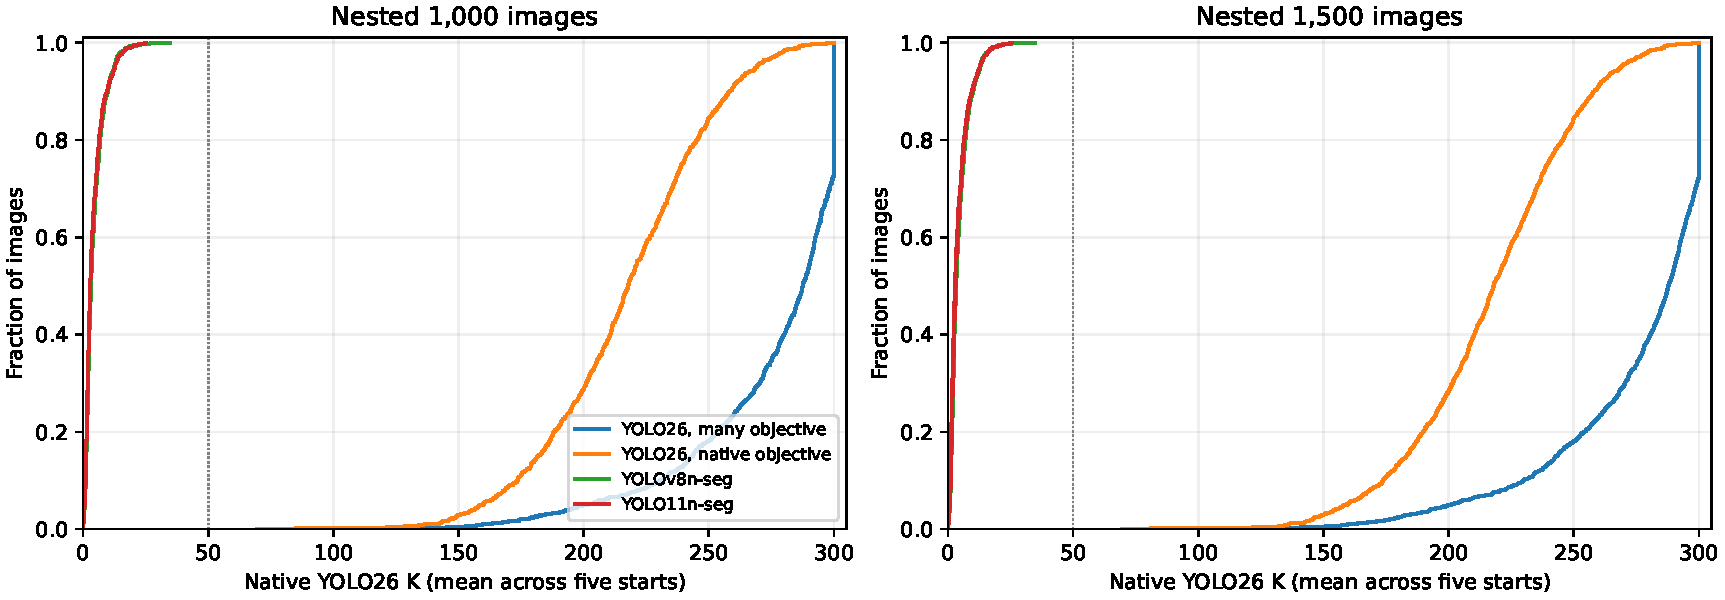
\includegraphics[width=\textwidth]{segmentation_extension/nested1500_native.pdf}\caption{Native YOLO26 count distributions under both transfer sources and both target-specific objectives. Each image contributes its mean count over five starts.}\label{fig:nested1500}\end{figure*}
Every case retains candidate-score vectors, detections, and native outputs. Exact adversarial inputs are retained only for the prospectively selected 64-image audit subset across all objectives and starts; the remaining cases have input hashes and saved-output verification, not full input replay. These count results do not repair the failed timing quality gates and do not establish an end-to-end denial of service.
